\chapter{Methods}
\label{c:method}

In the following sections, first a number of typical RNA-Seq and DNA-Seq
pipelines that BioCloud supports are defined and explained. Then the design of
BioCloud is explained by breaking down into two main parts: the website and the
report generator. For the website, the components including account
registration, data sources management, experiment design, and pipeline
execution are described and their roles are illustrated in the website overview
workflow. For the report generator, the workflow is shown to demonstrate how
outputs of each tool is extracted, parsed, and rendered into pre-defined
web-based report templates.



\section{RNA-Seq pipelines}

The RNA-Seq analysis pipelines that BioCloud supports are summarized in
Figure~\ref{fig:rnaseq-pipeline}, where some of the tools are shared for
different pipelines. The goal of RNA-Seq analysis is to infer differential
expression of gene or transcripts across different conditions. Based on
different assumptions of the distribution of gene and transcript expression,
three different methods are used: Cufflinks, DESeq2, and kallisto, which yield
FPKM based, count-based, and abundance-based expression value.

\begin{figure}[!htbp]
\centering
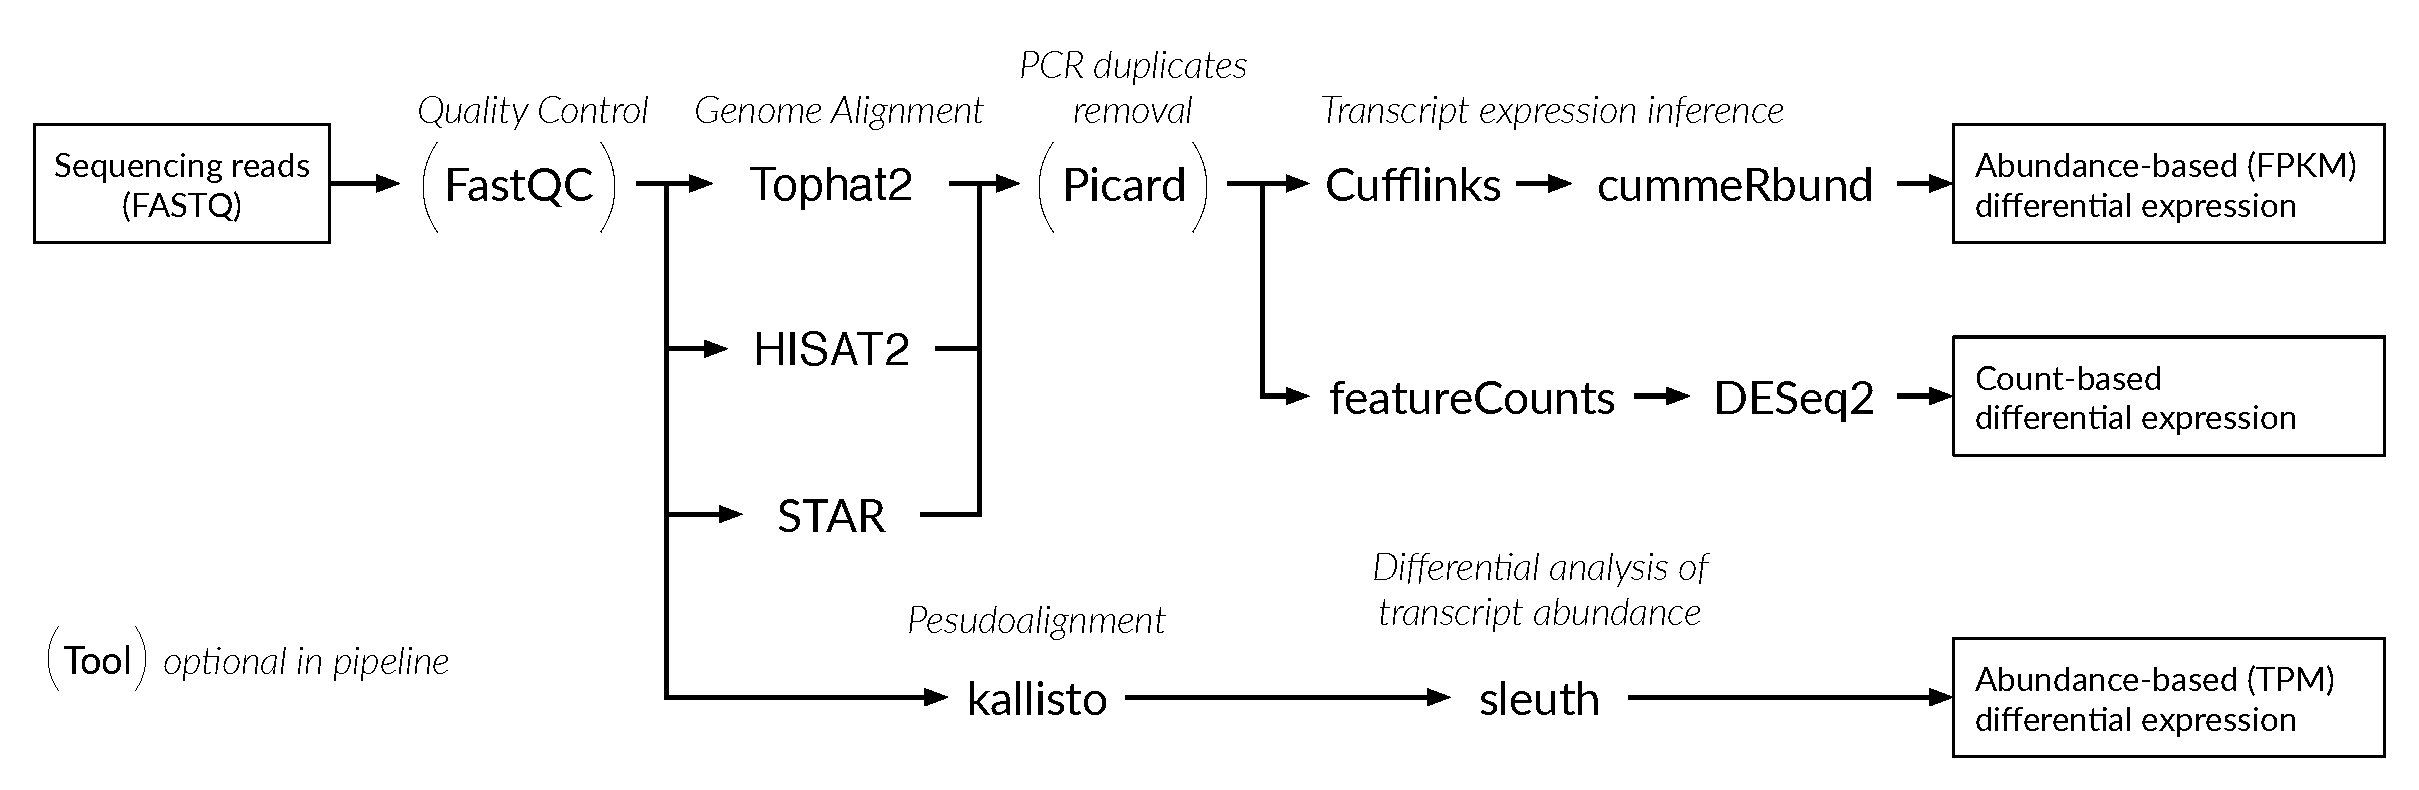
\includegraphics[width=\textwidth]{images/rnaseq_pipelines}
\caption[RNA-Seq analysis pipelines]{RNA-Seq analysis pipelines supported by BioCloud.}
\label{fig:rnaseq-pipeline}
\end{figure}


Cufflinks \cite{trapnell2010:transcript} and its differential analysis method
Cuffdiff \cite{trapnell2013:differential} are best used for gene expression
considering its isoforms, e.g., differential expression on transcript-level.
The output of Cuffdiff can be further visualized using R package cummeRbund
\cite{:cummerbund} from the same development team of Cufflinks. The unit of
expression Cufflinks uses is reads per kilobase of exon per million reads
mapped (FPKM). For DESeq2 \cite{love2014:moderated}, its model analyzes
expression change on gene level using read counts, which cannot be applied to
transcript level analysis. The unit of expression DESeq2 uses is normalized
read counts. The read counts are computed by featureCounts
\cite{liao2014:featurecounts}.  Another popular alternative for computing read
counts is HTSeq \cite{anders2015:htseqa}. HTSeq generally acts the same as
featureCoutns while having slower processing speed so it is not used in
BioCloud.

Both Cufflinks and DESeq2 require genomic location of reads so their analysis
is prepended by the genome alignment step. Three aligners are supported:
Tophat2 \cite{kim2013:tophat2}, HISAT2 \cite{kim2015:hisat}, and STAR
\cite{dobin2013:star}. Though the underlying alignment algorithms are
different, their alignment output in BAM file format can be used by the
following expression inference tools interchangeably. The most discernible
difference is computation time. Given the same execution environment on a same
sequencing sample, Tophat2 takes a hundred times the computation time of STAR
to complete the alignment. HISAT2 uses even slighter shorter time and
significantly less memory than STAR.



The analysis accepts raw sequence reads in
FASTQ format.



FastQC \cite{:fastqc}






Picard \cite{:picard}


kallisto \cite{bray2016:nearoptimal}

sleuth \cite{pimentel2016:differential}


\section{DNA-Seq pipelines}

The DNA-Seq analysis pipelines that BioCloud supports are summarized in
Figure~\ref{fig:dnaseq-pipeline}.

\begin{figure}[!htbp]
\centering
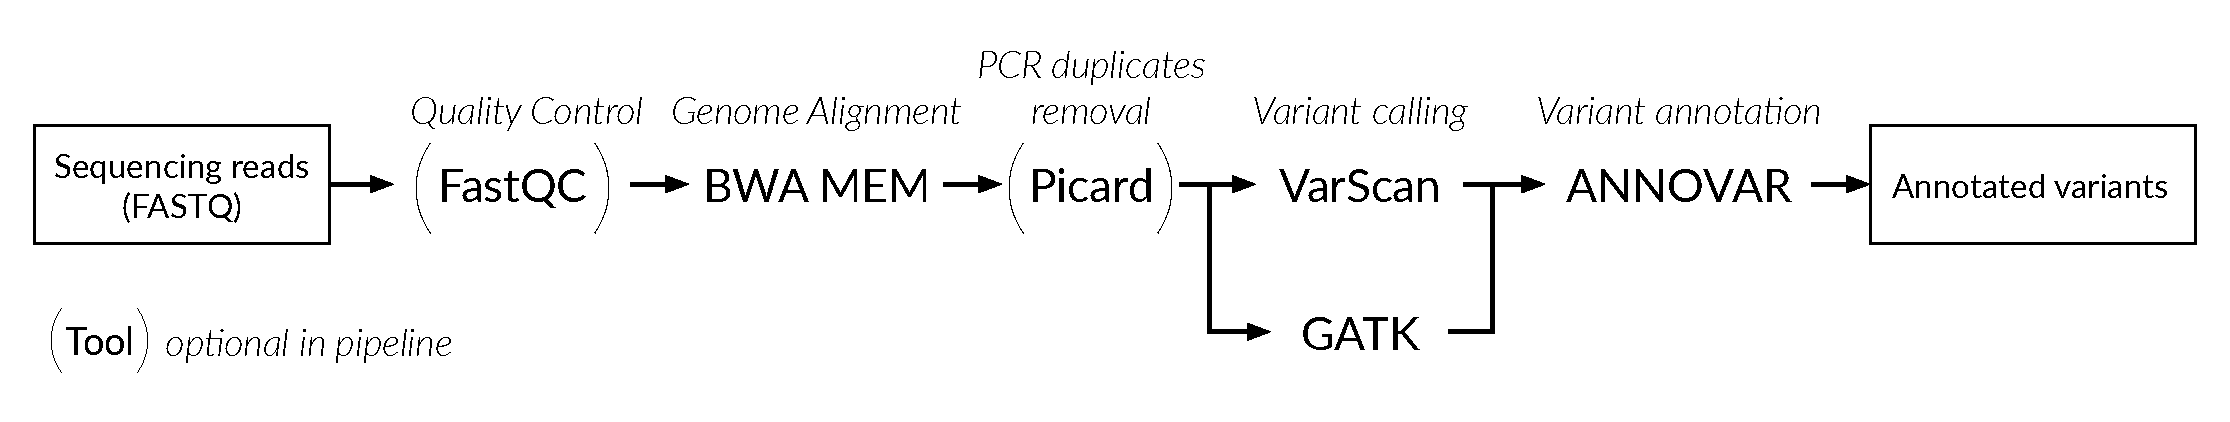
\includegraphics[width=\textwidth]{images/dnaseq_pipelines}
\caption[DNA-Seq analysis pipelines]{DNA-Seq analysis pipelines supported by BioCloud.}
\label{fig:dnaseq-pipeline}
\end{figure}




\section{Website workflow}

\begin{figure}[htbp]
\centering
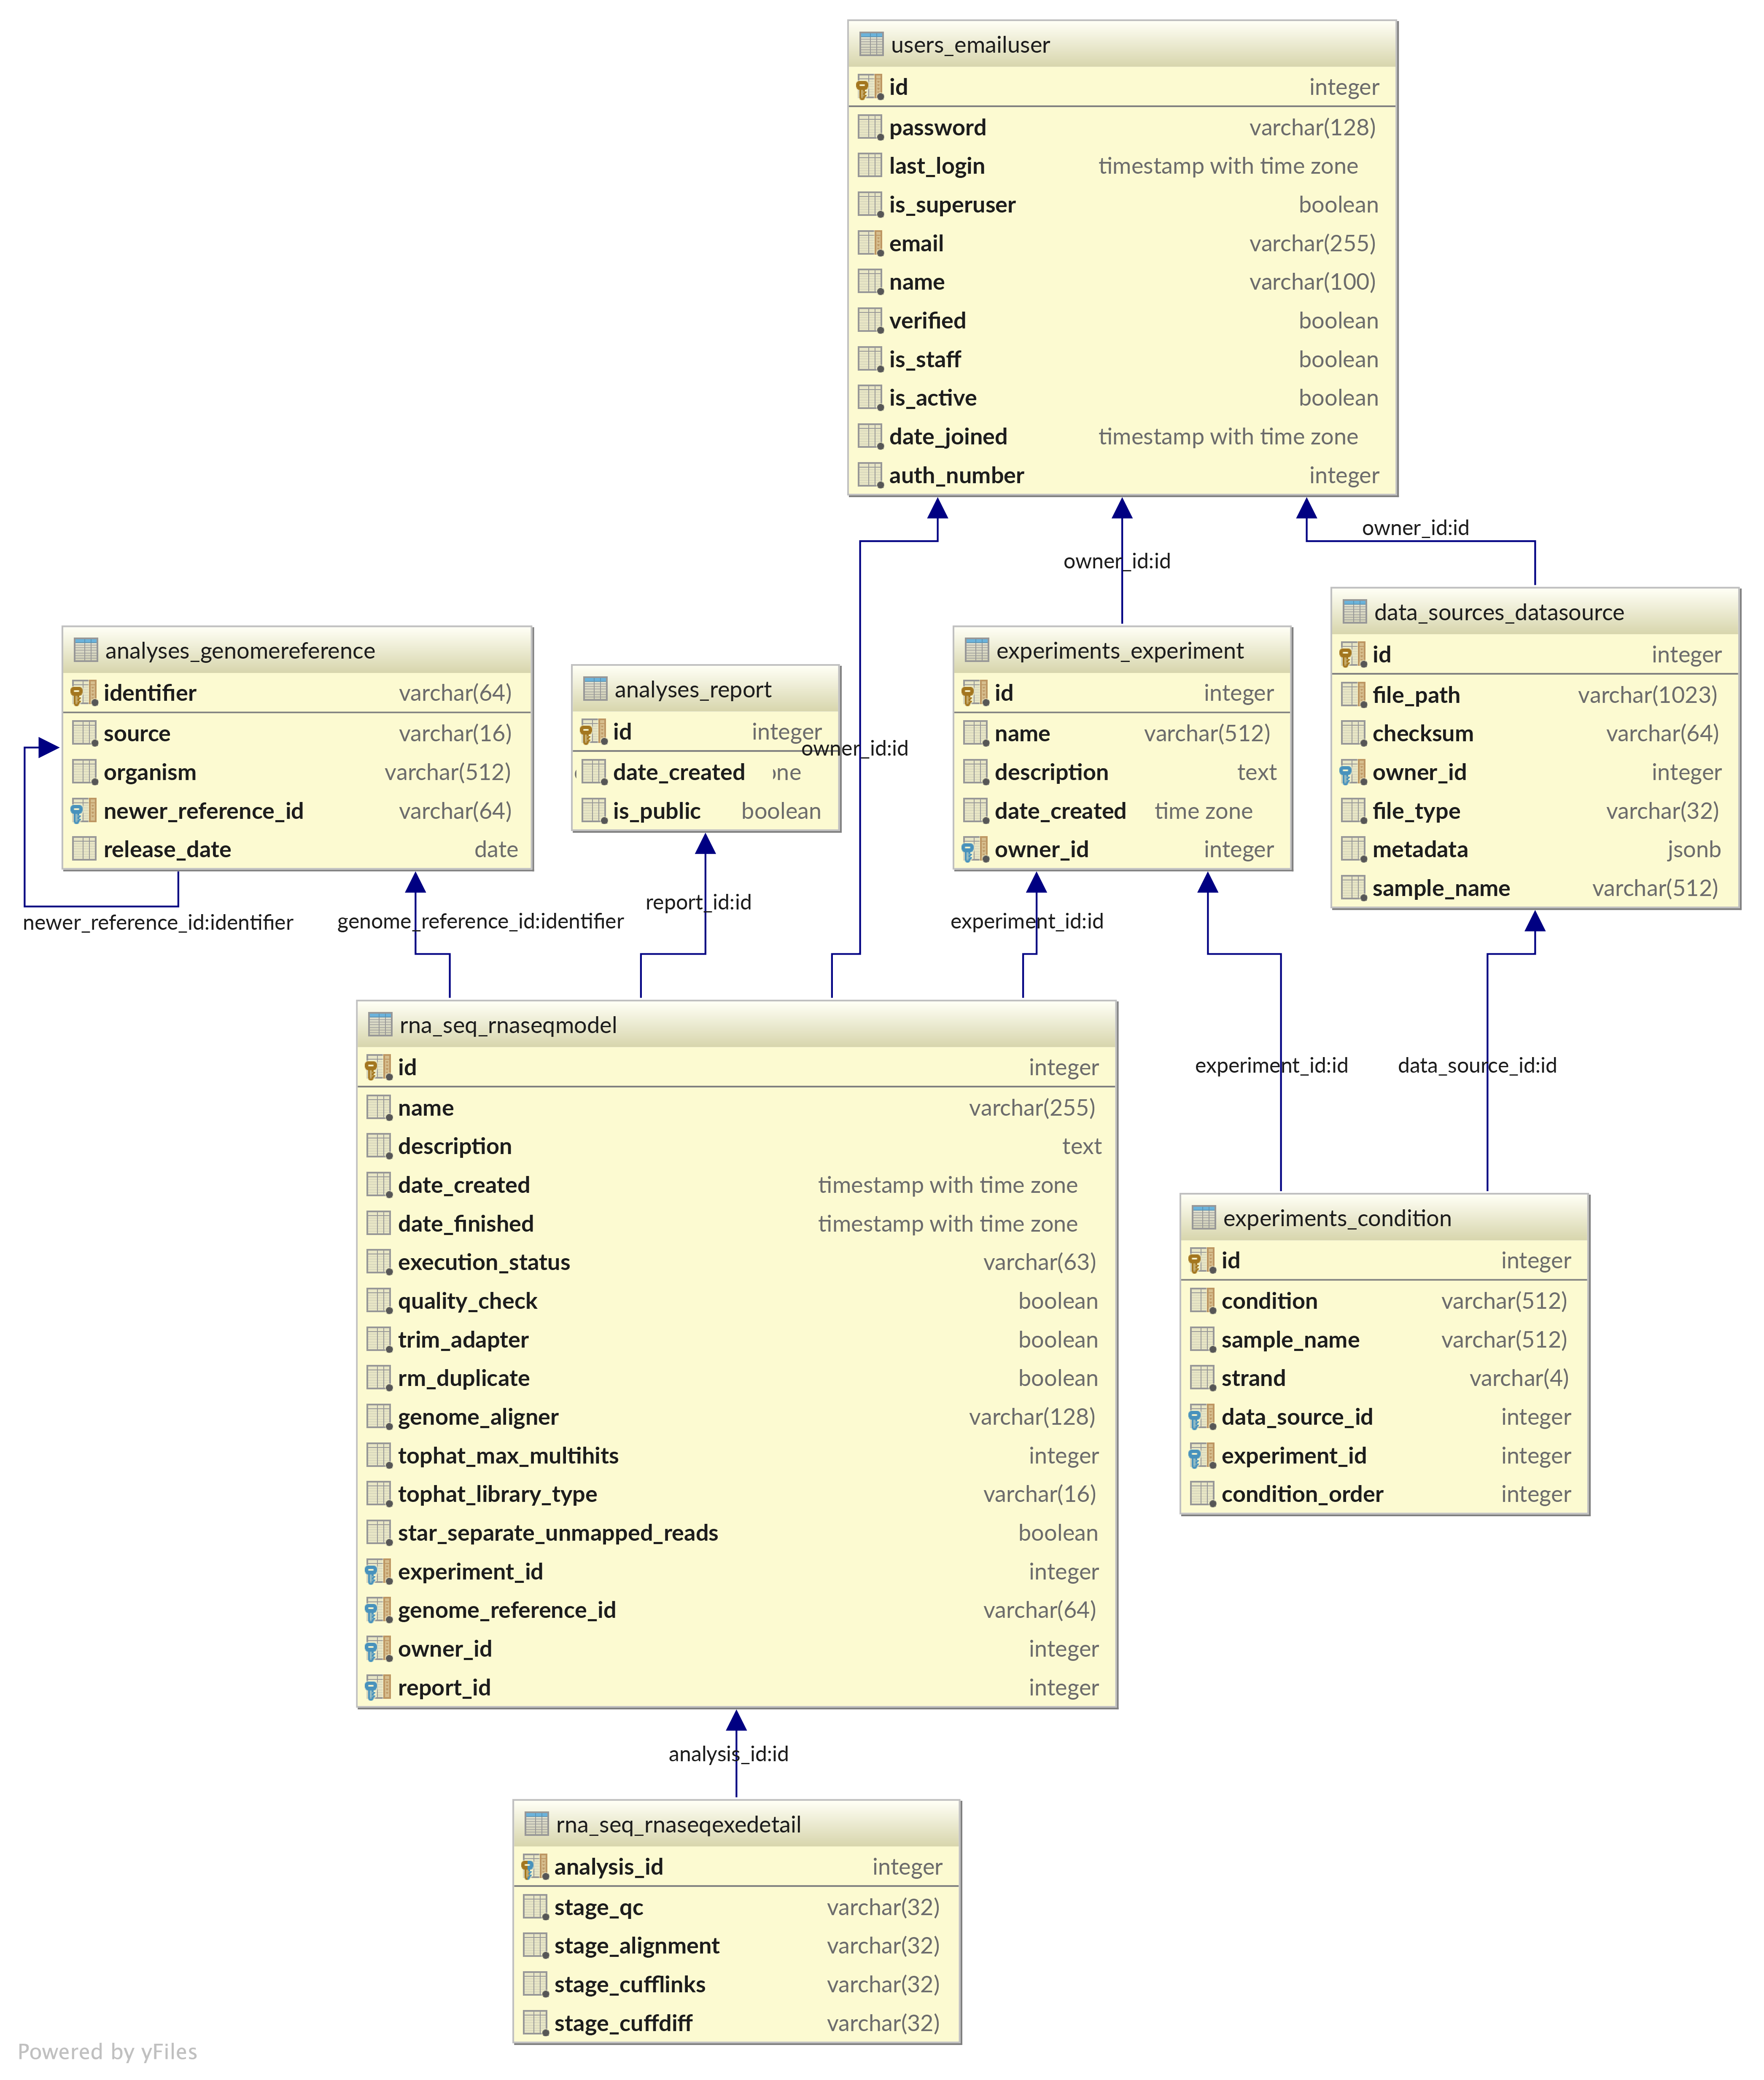
\includegraphics[width=\textwidth]{images/biocloud_erd}
\caption[Entity relation diagram (ERD) of BioCloud database]{
    Entity relation diagram (ERD) of BioCloud database. Here only one analysis
    pipeline of RNA-Seq (table \texttt{rna\_seq\_rnaseqmodel}) is shown for
    simplicity. Tables related with Django web framework internals and job
    queue framework are also omitted.
}
\label{fig:biocloud-erd}
\end{figure}


\subsection{Overall design}

\subsection{Message authentication and checksum}

Hash-based message authentication code (HMAC)

\subsection{HMAC-based account registration}

\subsection{Experiement design}

\subsection{Genome reference}

\subsection{Analysis submission}

\subsection{Job queue management}

\subsection{Report and result access control}



\section{Report generation}

\subsection{BCReport: result processing framework}



\section{Implementation}

\subsection{Website}

\subsection{Deployment}

\subsection{Report}
% vim: set textwidth=79:
